\section{Physics Package based on Coherent Population Trapping (CPT)}
% CPT (Coherent Population Trapping) (theory -> physical components -> VCSEL

\begin{frame}{Superposition of Quantum States (concept)}

    Before exploring the CPT itself, it's important to understand the concept of superposition of quantum states by using the Bloch sphere representation.

    \begin{columns}

        \begin{column}{0.32\textwidth}

            \onslide<2->{
                \begin{figure}
                    \centering
                    \includegraphics[width=0.9\textwidth]{pdf/states/ground-state.pdf}
                    \caption{Ground state}
                \end{figure}
            }

        \end{column}

        \begin{column}{0.32\textwidth}

            \onslide<4->{
                \begin{figure}
                    \centering
                    \includegraphics[width=0.9\textwidth]{pdf/states/superposition-state.pdf}
                    \caption{Superposition of states}
                \end{figure}
            }

        \end{column}

        \begin{column}{0.32\textwidth}

            \onslide<3->{
                \begin{figure}
                    \centering
                    \includegraphics[width=0.9\textwidth]{pdf/states/excited-state.pdf}
                    \caption{Excited state}
                \end{figure}
            }

        \end{column}

    \end{columns}

    \onslide<3->{
        \begin{figure}

            \centering

            \resizebox{\columnwidth}{!}{%
                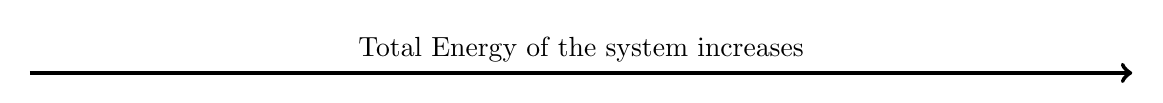
\begin{tikzpicture}[scale=0.5]
                    \draw[ultra thick, ->] (0,0) -> (28,0) node[midway, above] {Total Energy of the system increases};
                \end{tikzpicture}
            }

        \end{figure}
    }

\end{frame}



\begin{frame}{Dark state \& $\Lambda$-system}

    \textit{"In atomic physics, a dark state refers to a state of an atom or molecule that cannot absorb (or emit) photons."}

    \begin{columns}[T, onlytextwidth]

        \begin{column}{0.45\textwidth}

            \begin{figure}
                \centering
                \includegraphics[width=\textwidth]{pdf/lambda-system.pdf}
                \caption{$\Lambda$-system.}
            \end{figure}

        \end{column}

        \begin{column}{0.55\textwidth}

            \vspace{30pt}

            \begin{align}
                \text{Allowed transitions:}  & \begin{cases}
                                                   \ket{1} \leftrightarrow \ket{3} \\
                                                   \ket{2} \leftrightarrow \ket{3}
                                               \end{cases} \\
                \text{Forbidden transition:} & \begin{cases}
                                                   \ket{1} \leftrightarrow \ket{2}
                                               \end{cases}
            \end{align}

        \end{column}

    \end{columns}

    \vspace{10pt}

    In this case the dark state happens to be a superposition of $\ket{1}$ and $\ket{2}$.

\end{frame}



\begin{frame}{$^{133}Cs$ Reference Cell}

    At the heart of a CPT based CSAC, we find a $^{133}Cs$ reference cell.

    \vspace{10pt}

    \begin{columns}[c, onlytextwidth]

        \begin{column}{0.45\textwidth}

            \begin{figure}
                \centering
                \only<1>{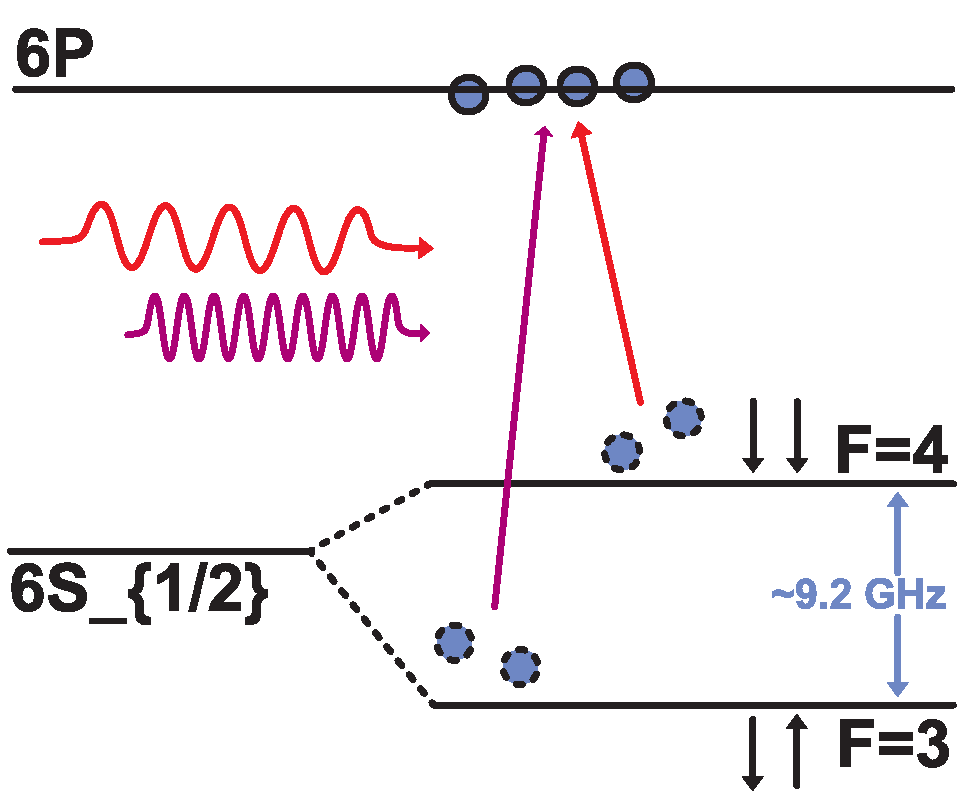
\includegraphics[width=0.9\textwidth]{pdf/CPT/pumping.pdf}}
                \only<2>{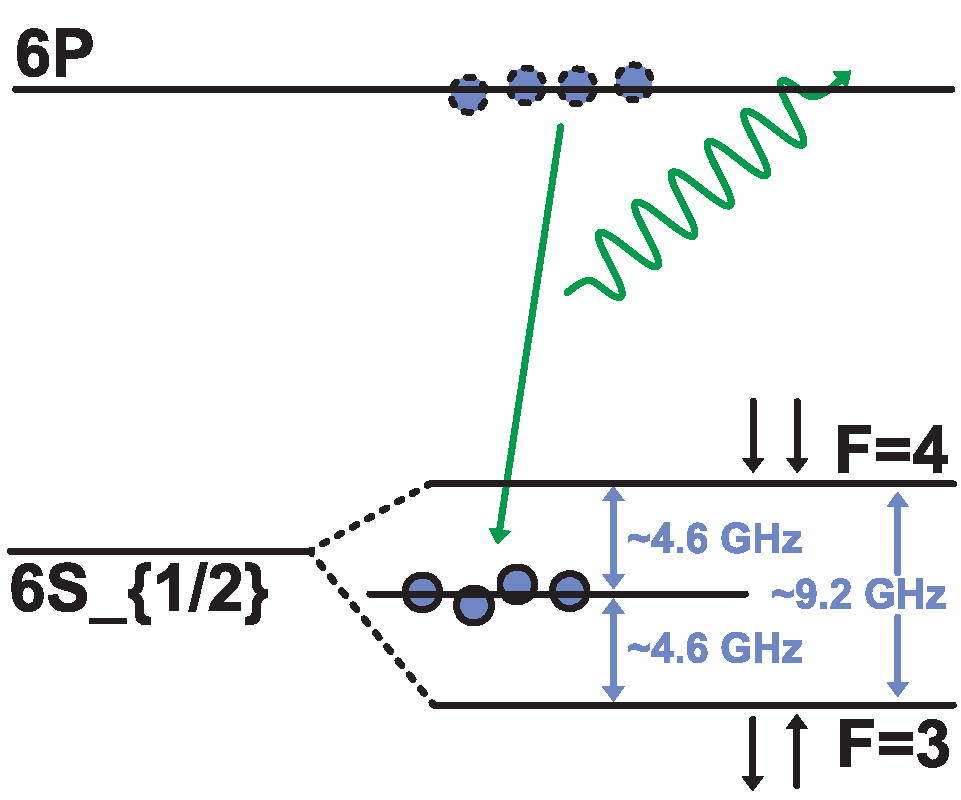
\includegraphics[width=0.9\textwidth]{pdf/CPT/decay.pdf}}
                \only<3>{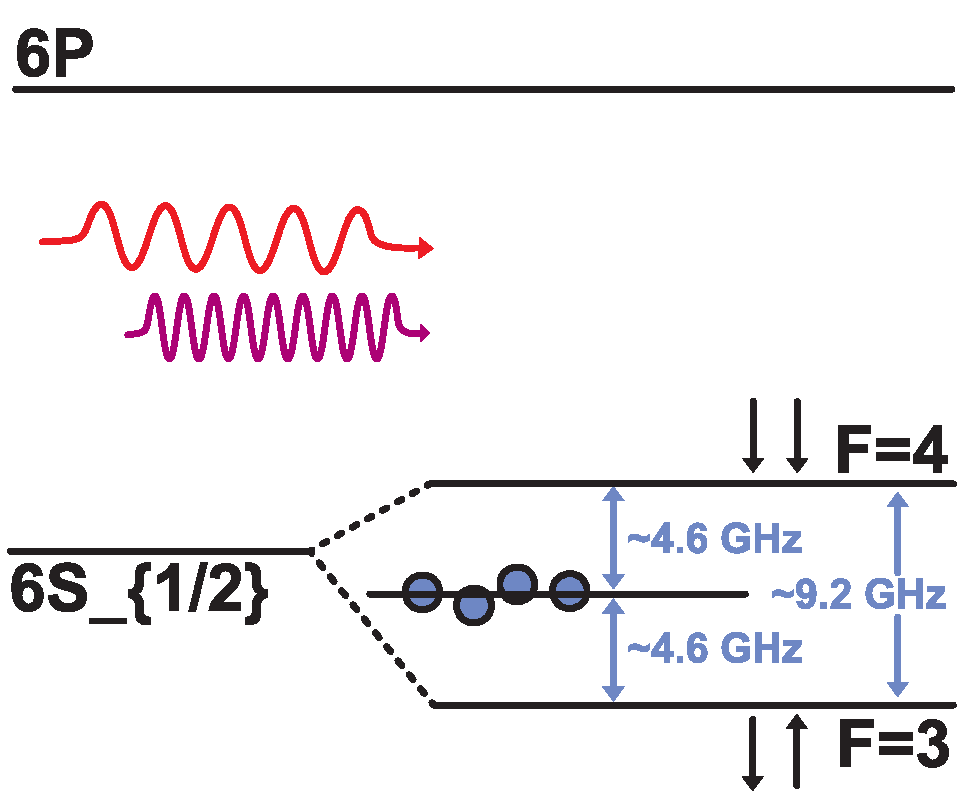
\includegraphics[width=0.9\textwidth]{pdf/CPT/interrogation.pdf}}
            \end{figure}

        \end{column}

        \begin{column}{0.55\textwidth}

            We can distinguish 3 processes:

            \begin{enumerate}
                \item<1-> \textbf<1>{Optical Pumping (Population Inversion)}
                \item<2-> \textbf<2>{Decay to the dark state (superposition state)}
                \item<3-> \textbf<3>{Optical Pumping (Interrogation)}
            \end{enumerate}

        \end{column}

    \end{columns}

    \vspace{10pt}

    \only<1>{A dual-frequency laser is used to pump the population from both $F=\ket{1}$ and $F=\ket{2}$ to $6P$.}
    \only<2>{
        Because of the particular beat frequency and phase of the laser, the population will (over time) fall into a superposition state.

        \begin{equation}
            \ket{\psi} = \ket{Dark} = \frac{1}{\sqrt{2}} \left( \ket{3} + \ket{4} \right)
        \end{equation}
    }
    \only<3>{
        Being in a superposition state $\ket{\psi}$, the population will not absorb the pumping laser radiation anymore.
        \textbf{Electrons are now trapped.}
    }

\end{frame}



\begin{frame}{Photodetection}

    At the end of the cell, a photodiode is used to measure the intensity of the transmitted radiation.

    \begin{columns}[c, onlytextwidth]

        \begin{column}{0.45\textwidth}

            \begin{figure}
                \centering
                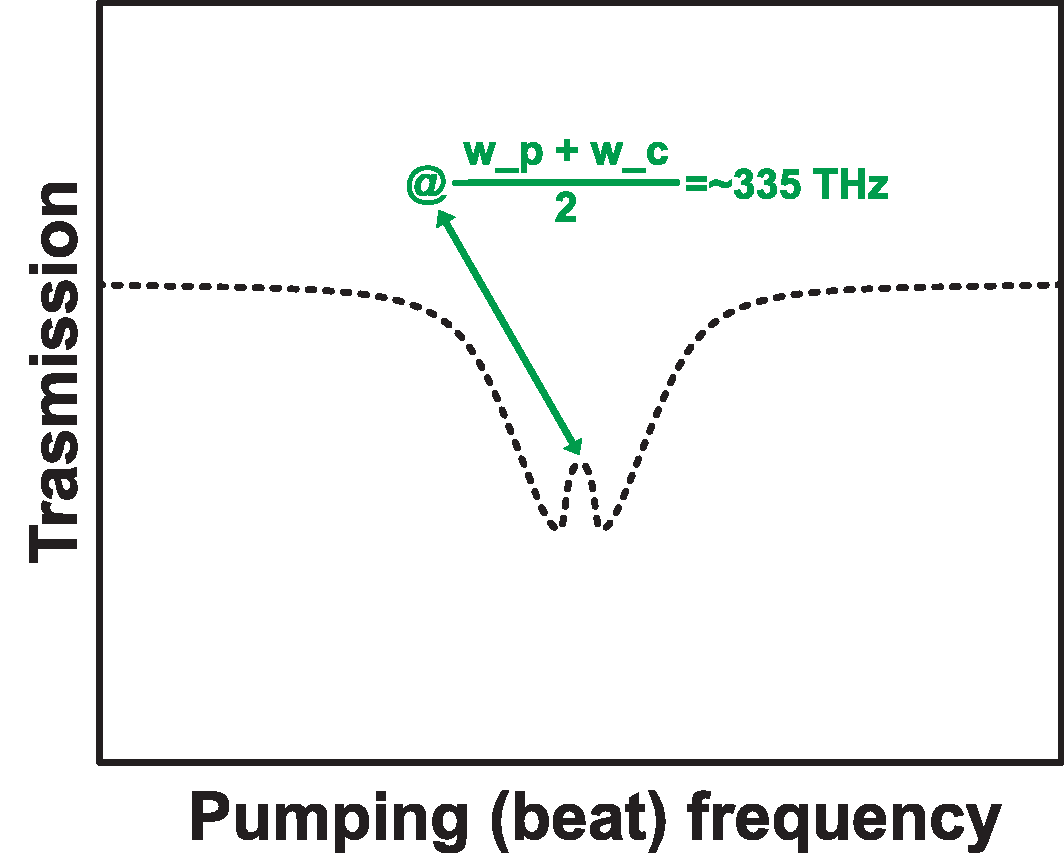
\includegraphics[width=0.9\textwidth]{pdf/CPT-trasmission-curve.pdf}
            \end{figure}

        \end{column}

        \begin{column}{0.55\textwidth}

            \begin{figure}
                \centering
                \includegraphics[width=0.9\textwidth]{pdf/beating-waves.pdf}
            \end{figure}

        \end{column}

    \end{columns}

    \vspace{10pt}

    Our target is to stay at the peak in the middle of the valley in the transmission curve.
    % Notice how that point is associated to a laser frequency of $\approx 4.6 GHz$ in case of $^{133}Cs$.

\end{frame}



\begin{frame}{Complete Physics Package for a CPT-based CSAC}

    \begin{columns}[c, onlytextwidth]

        \begin{column}{0.35\textwidth}

            \begin{figure}
                \centering
                \includegraphics[width=\textwidth]{img/CPT-physics-package-1.png}
            \end{figure}

        \end{column}

        \hfill

        \begin{column}{0.6\textwidth}

            Power consumption\footnotemark[1]: $\approx 10mW$.

            Volume: $\approx 0.35 cm^3$.

            \vspace{10pt}

            \begin{figure}

                \centering
                \only<1>{\includegraphics[width=0.7\textwidth]{img/CPT-physics-package-2.png}}
                \only<2>{
                    \includegraphics[width=0.5\textwidth]{img/CPT-physics-package-3.png}
                    \caption{Microchip SA.45s physics package.}
                }

            \end{figure}

            \footnotetext[1]{The entire package is vacuum sealed to minimize the heating power required (to stabilize).}
            \footnotetext[2]{LCC: Leadless Chip Carrier.}
            \footnotetext[3]{VCSEL: Vertical-Cavity Surface-Emitting Laser.}

        \end{column}

    \end{columns}

\end{frame}



\begin{frame}{Vertical-Cavity Surface-Emitting Laser (VCSEL)}

    % VCSEL, schematics, importance of its stability.

    % Flexibilty in the choice of the optical wavelength (allowance for both Rb and Cs).

    % ~ power consumption (from travaglin @36)

    VCSELs are a type of semiconductor laser diode with laser beam emission perpendicular to the chip surface.

    \begin{figure}
        \centering
        \includegraphics[width=0.6\textwidth]{img/CPT-VCSEL.png}
    \end{figure}

    In CPT-based CSACs, the VCSEL is used as the radiation source:

    \begin{itemize}
        \item Stability in the emitted frequency.
        \item Flexibility in the choice of the optical wavelength.
        \item Low power consumption ($\approx 3mW$).
    \end{itemize}

\end{frame}


\begin{frame}{Design bottleneck}

    CPT-based CSACs partially solve the bottleneck of size and power consumption of the MODR-based CSACs.

    \vspace{10pt}

    Still, we can recognize some area of improvements:

    \begin{itemize}
        \item Working temperature range\footnotemark[1] (currently $\approx [-40; 80]^{\circ}C$).
        \item High sensitivity to temperature and voltage fluctuations.
        \item Short-term frequency stability (currently $\approx 3 \times 10^{-10}@\tau=1s$).
    \end{itemize}

    \footnotetext[1]{Mainly due to degradation in performance of the resonance cell (buffer gas pressure).}

\end{frame}